\documentclass{beamer}
%\mode<presentation>
\usepackage[utf8]{inputenc}
\usepackage[magyar]{babel}
\usetheme{CambridgeUS}
\usecolortheme{dolphin}
\usepackage{amsmath,amssymb,amsfonts, bm}
\usepackage{mathpazo}
\usepackage{graphicx,tabularx,epsfig}
\usepackage[compatibility=false]{caption}
\usepackage{subcaption}
\usepackage{rotating}


\setbeamertemplate{background}{\tikz[overlay,remember picture]\node[opacity=0.2]at (current page.center){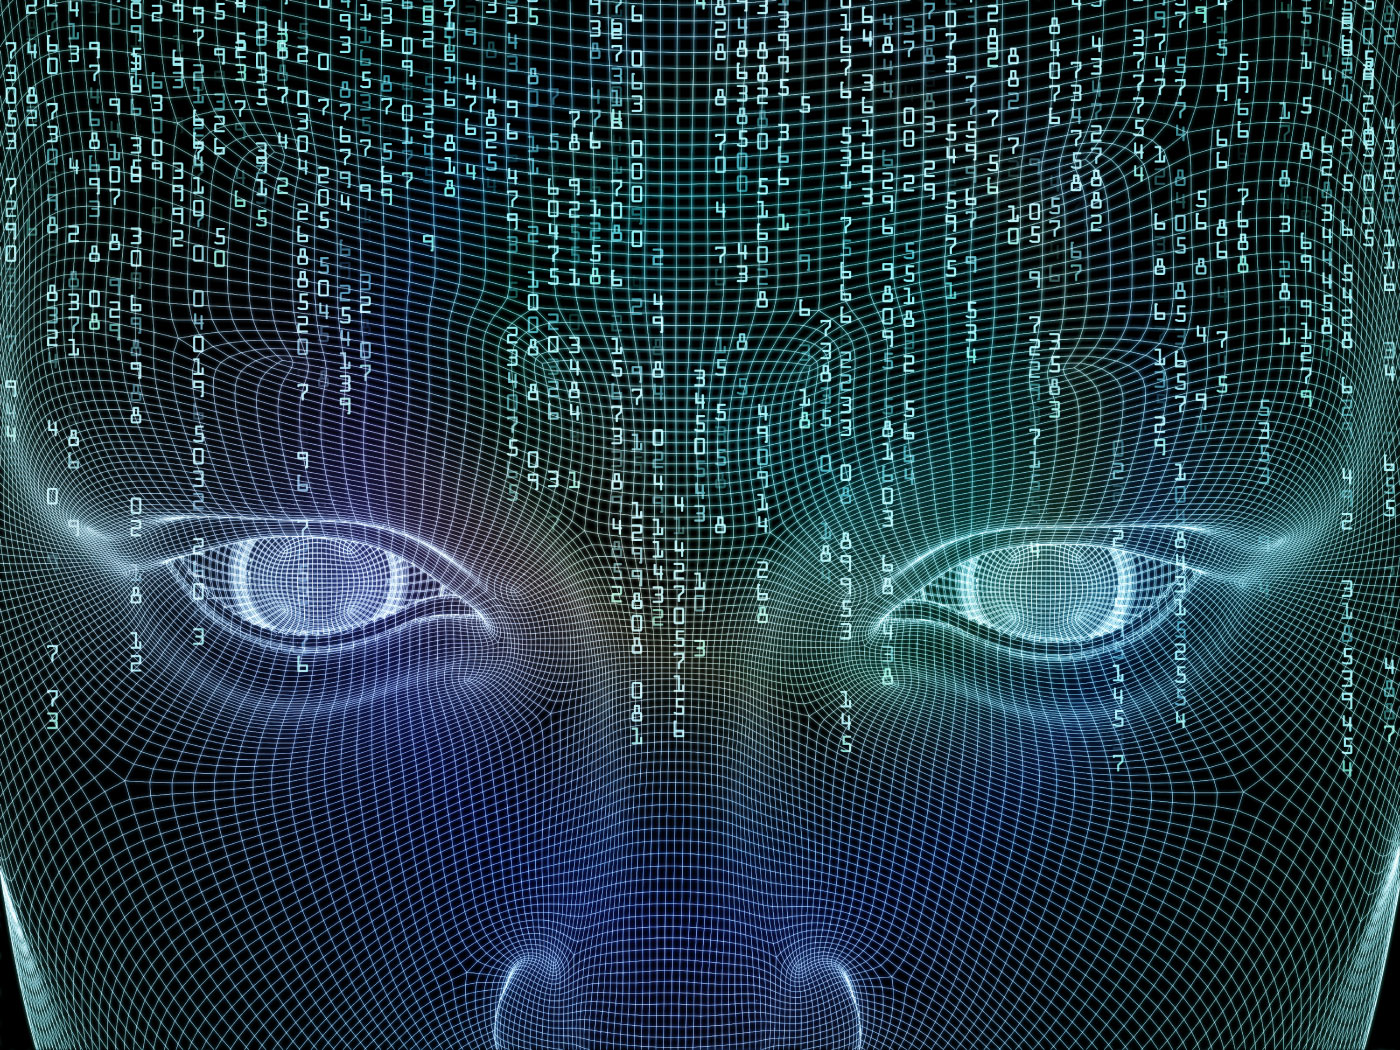
\includegraphics[width=\paperwidth]{pic/bkg}};}
\usepackage{tikz}

\DeclareGraphicsExtensions{.pdf,.png,.jpg,.svg}


\setbeamertemplate{itemize items}[square]
\setbeamertemplate{enumerate items}[square]

\definecolor{Red}{RGB}{190,0,0}
\definecolor{Blue}{RGB}{0,0,190}
\setbeamertemplate{headline}{}



\title[Machine learning]{Neuronhálózatok a részecskefizikában}
\author[Bagoly Attila]{Bagoly Attila\\ ELTE TTK Fizikus MSc, 2. évfolyam \vspace{0.5cm}}
\date[2016.10.10.]{2016.10.10}
\institute[ELTE]{
\large{Integrating Machine Learning in Jupyter Notebooks}
\begin{figure}[H]
	\centering
    
\includegraphics[height=40pt]{pic/CERN-Logo}
	
\includegraphics[height=40pt]{pic/gsoc_project}
\end{figure}
}

\begin{document}

\begin{frame}
  \titlepage
\end{frame}

\begin{frame}
\frametitle{Tartalom}
\tableofcontents
\end{frame}



\section{Bevezető}
\begin{frame}
\frametitle{Bevezető}
\begin{itemize}
  \setlength{\itemsep}{10pt}
\item Nagyon magas dimenziós problémákra, komplex modellt szeretnénk
\item "Klasszikus illesztés": nem működik
\item Probléma "megkerülése": neuronhálózatok
\item Klasszifikáció: modell kimenete diszkrét (valahány osztályba sorolás)
\item DNN manapság népszerű: erős számítógép (GPU), sok adat
\item Machine learning: hihetetlenül gyorsan fejlődő terület
\item DNN: része mindennapjainknak
\item HEP-ben is egyre népszerűbb: CERN IML(\url{http://iml.web.cern.ch/}), tagok száma 100-as nagyságrend
\item CMS L1 trigger: boosted decision tree hardver
\end{itemize}
\end{frame}

\section{Lineáris regresszió}
\begin{frame}
\frametitle{Lineáris regresszió}
\begin{itemize}
  \setlength{\itemsep}{12pt}
  \item Mindenki által ismert "egyszerű" függvényillesztés
  \item $x_j^{(i)}$ a j-edik változó az i-edik adatsorban
  \item Modell: $h_\Theta(x)=\Theta_0+\Theta_1x_1+\Theta_2x_2+...$
  \item Nem feltétlenül lineáris: $x_j$ kiegészíthető, ha $j=1...N$ akkor $x_{N+k}=x_k^2$, stb.
  \item nem linearitás $\Rightarrow$ magasabb dimenziós lineáris illesztés
  \item Költségfüggvény: $J(\Theta) = \frac{1}{2m}\sum_{i=1}^{m}(h_\Theta(x^{(i)})-y^{(i)})^2$
  \item Minimalizálás: pl. gradiens módszer $\Theta\leftarrow\Theta-\alpha\Delta J(\Theta)$
\end{itemize}

\end{frame}

\section{Logisztikus regresszió}
\begin{frame}
\frametitle{Logisztikus regresszió}
\begin{minipage}{0.48\textwidth}
\begin{itemize}
  \setlength{\itemsep}{16pt}
\item Klasszifikáció?
\item Diszkrét kimenet
\item Két kategória: 0 vagy 1
\item $h_\Theta(x)$ tetszőleges kimenetet vehet fel $\Rightarrow$ beszorítjuk 0 és 1 közé
\item Sigmoid aktivációs függvény: $\mathrm{sigmoid}(x)=\frac{1}{1+e^{-x}}$
\end{itemize}
\end{minipage}
\begin{minipage}{0.48\textwidth}
\begin{figure}
\centering
	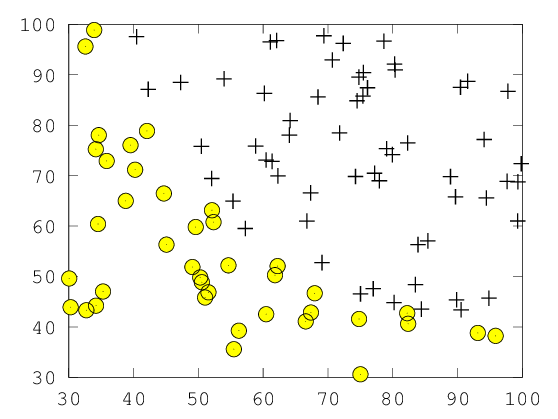
\includegraphics[scale=0.55]{pic/nn/1}\\
	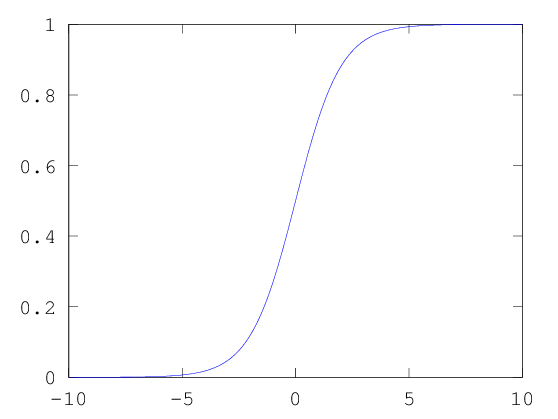
\includegraphics[scale=0.55]{pic/nn/2}
\end{figure}
\end{minipage}
\end{frame}

\begin{frame}
\frametitle{Logisztikus regresszió}
\begin{itemize}
  \setlength{\itemsep}{12pt}
  \item Mi a modell költségfüggvénye?
  \item Tudnia kell: 
  	\begin{itemize}
  		\item Ha $h_\Theta(x)=y$ akkor $0$
  		\item Ha $h_\Theta(x)=1$ és $y=0$ akkor nagy
  		\item Ha $h_\Theta(x)=0$ és $y=1$ akkor nagy
  	\end{itemize}
  \item Egyszerű választás:
\begin{equation*}
J(\Theta)=- \frac{1}{m} \displaystyle \sum_{i=1}^m [y^{(i)}\log (h_\theta (x^{(i)})) + (1 - y^{(i)})\log (1 - h_\theta(x^{(i)}))]
\end{equation*}
\item N kategória esetén: 
	$ y \in \lbrace0, 1 ... N-1\rbrace $ \\
	$h_\theta^{(0)}(x) = P(y = 0 | x ; \theta)$\\
	$h_\theta^{(1)}(x) = P(y = 1 | x ; \theta)$\\ ...\\
	$\mathrm{pred} = \max_i( h_\theta ^{(i)}(x) )$
\end{itemize}

\end{frame}


\begin{frame}
\frametitle{Logisztikus regresszió}
\begin{itemize}
  \setlength{\itemsep}{12pt}
  \item Lineáris modell: $x_1, x_2$, $h_\Theta(x) = \mathrm{sigmoid}(\Theta_0+\Theta_1x_1+\Theta_2x_2)$
  \item Nem lineáris modell: $x_1, x_2$ featureket kiegészítjük $x_3=x_1^2, x_4=x_2^2, x_5=x_1x_2$, és $x_0=1$, ekkor $h_\Theta(x)=\mathrm{sigmoid}(\Theta^T x)$
\end{itemize}
\begin{figure}[H]
	\centering
    \begin{subfigure}[b]{0.49\textwidth}
    		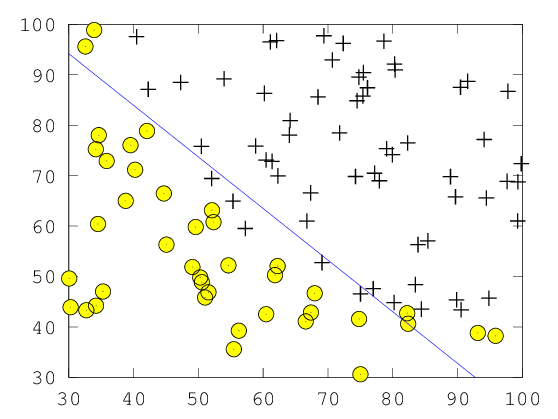
\includegraphics[width=\textwidth]{pic/nn/3}
	\end{subfigure}
	\begin{subfigure}[b]{0.49\textwidth}
        	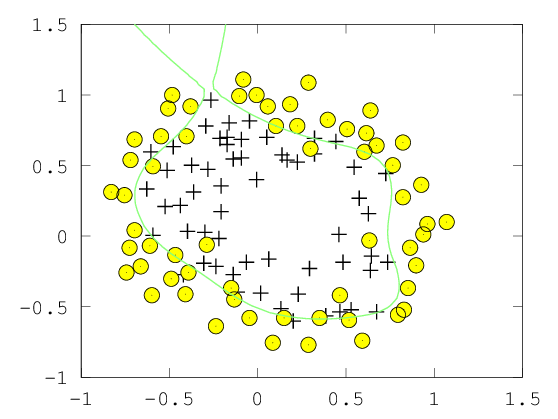
\includegraphics[width=\textwidth]{pic/nn/4}
	\end{subfigure}
\end{figure}
\end{frame}

\begin{frame}
\frametitle{Hogy általánosít a modellünk?}
\begin{itemize}
  \setlength{\itemsep}{6pt}

\item Hogy teljesít a modellünk? Nem lineáris problémánál 2D$\Rightarrow$5D
\item $J(\Theta)$ hiba kicsi, jó az illesztés?
\item $J(\Theta)$ kicsi mégis új adatra teljesen rossz eredmény $\Rightarrow$ nem modelleztünk hanem adatokat kódoltunk (overfit, high variance)
\item Kevés feature: underfit, high bias
\begin{figure}[H]
	\centering
    		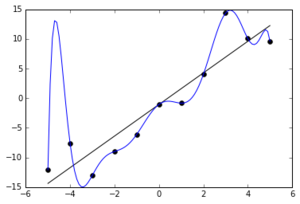
\includegraphics[width=0.6\textwidth]{pic/nn/5}
\end{figure}
\end{itemize}
\end{frame}

\section{Illesztés jellemzése}
\begin{frame}
\frametitle{Megoldás}
\begin{minipage}{0.48\textwidth}

\begin{itemize}
  \setlength{\itemsep}{6pt}
\item Felosztjuk az adatokat: training set, test set
\item Fontos: adatok random keverve legyenek
\item Csak az egyiken tanul a modellünk
\item Probléma: paraméterek csavargatásával a modell a szemünkön keresztül tanulja meg a test set-et
\item Megoldás: k-fold Cross-Validation
\end{itemize}
\end{minipage}
\begin{minipage}{0.48\textwidth}

\begin{figure}[H]
	\centering
    		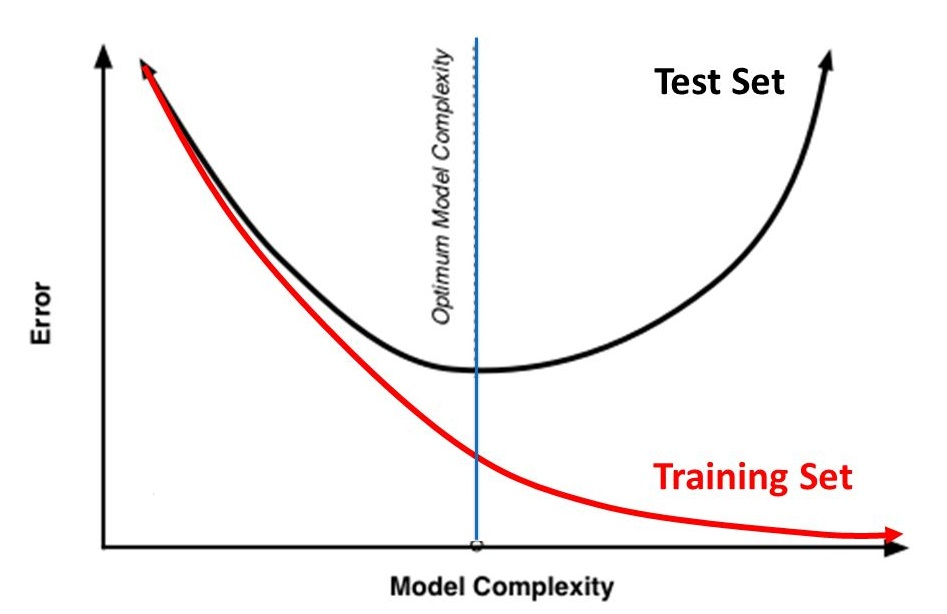
\includegraphics[width=\textwidth]{pic/nn/6}
\end{figure}
\end{minipage}
\end{frame}

\section{Problémák}
\begin{frame}
\frametitle{Problémák}
\begin{itemize}
  \setlength{\itemsep}{12pt}
\item Valós életben általában sokkal több feature van mint kettő
\item n változó, kvadratikus modell paramétereinek száma $\approx \mathcal{O}(n^2/2)$
\item Pl. 50x50 pixeles szürkeárnyalatos képeket osztályozunk $\Rightarrow$ 2500 változó $\Rightarrow$ 3125000 paraméter
\item Ráadásul kvadratikus modell valószínűleg high bias-t eredményez
\end{itemize}
\end{frame}

\section{Neuronhálózatok}
\begin{frame}
\frametitle{Neuronhálózatok bevezetés}
\begin{itemize}
  \setlength{\itemsep}{12pt}
\item Előbb vázolt probléma megoldására született
\item Lehetővé teszi nagyon komplex modell illesztését anélkül, hogy a paraméterek száma divergálna
\item Használjuk a nagyon egyszerű logisztikus modellt, de csak lineáris featurekkel $\Rightarrow$ Neuron
\item Sigmoid aktivációs függvény: neuron aktiválási valószínűség (agyban is hasonló a neuronok karakterisztikája)
\item Komplex modell: neuronokat összekötjük
\end{itemize}
\end{frame}

\begin{frame}
\frametitle{Neuronhálózatok}
\begin{figure}[H]
	\centering
    		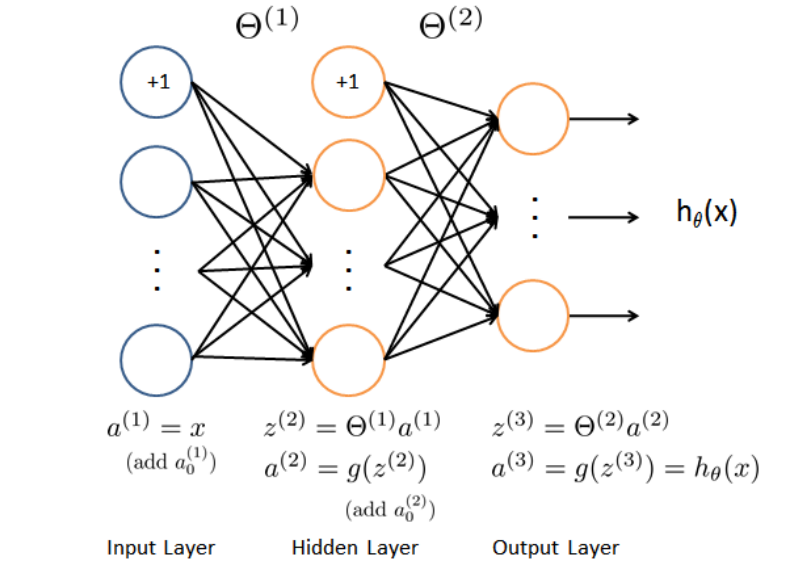
\includegraphics[width=\textwidth]{pic/nn}
\end{figure}
\end{frame}

\begin{frame}
\frametitle{Neuronhálózatok: bementet, kimenet}
\begin{itemize}
  \setlength{\itemsep}{18pt}
  \item Amennyi bemenet annyi neuron az első rétegben: minden bemenet minden neuronra kapcsolva
  \item Annyi kimeneti neuron az utolsó rétegben amennyi osztályunk van
  \item Minden kimeneti neuronok 0 1 közti értéket vesznek fel: a legnagyobb az adott adat osztálya
  
\end{itemize}
\end{frame}

\begin{frame}
\frametitle{Neuronhálózatok tanítása}
\begin{itemize}
  \setlength{\itemsep}{12pt}
  \item Költségfüggvény: csak össze kell rakni a logisztikus modellből
  \item Probléma: könnyű overfittelni neuronhálókkal
  \item Megoldás: regularizáció bevezetése: négyzetesen elnyomjuk a súlyokat valamilyen paraméterrel: $\lambda\sum_{i=1 (i\neq 0)}(\Theta_i)^2$, $\lambda\rightarrow 0$ overfitting, $\lambda\rightarrow\infty$ underfitting
  \item Tehát ezt kell minimalizálni:
    \begin{multline*}
\large J(\Theta) = - \frac{1}{m} \sum_{i=1}^m \sum_{k=1}^K [y^{(i)}_k \log ((h_\Theta (x^{(i)}))_k) + \\
 (1 - y^{(i)}_k)\log (1 - (h_\Theta(x^{(i)}))_k)] + 
  \frac{\lambda}{2m}\sum_{l=1}^{L-1} \sum_{i=1}^{s_l} \sum_{j=1}^{s_{l+1}} ( \Theta_{j,i}^{(l)})^2
\end{multline*}
\item $m$ adatpont, $K$ kategória, $s_l$ neuron az $l$-edik rétegben
\end{itemize}
\end{frame}

\begin{frame}
\frametitle{Neuronhálózatok tanítása}
\begin{itemize}
  \setlength{\itemsep}{12pt}
  \item Tehát neuronháló tanítása a fenti költségfüggvény minimalizálása
  \item Nem könnyű feladat, de elvégezhető
  \item Backpropagation algorithm:
  	\begin{itemize}
  		  \setlength{\itemsep}{6pt}

  	  		\item Előre propagálás: az adatokat végigvisszük a hálón, hogy megkapjuk a neuronok aktivációit
  	  		\item Hátra propagálás: aktivációkat és cél tanuló mintát visszafele propagáltatjuk a hálózaton, így kapunk egy delta mátrixot
  	  		\item Delta mátrix segítségével felírhatjuk a költségfüggvény deriváltját
  	  		\item Derivált alapján súlyokat frissítünk
  	\end{itemize}
  	\item Regularizációs paraméter optimumát is meg kell keresi (hyper parameter optimalization): k-fold coross-validation pár csoport hibái alapján
\end{itemize}
\end{frame}

\section{Mély neuronhálózatok}
\begin{frame}
\frametitle{Mély neuronhálózatok}
\begin{minipage}{0.48\textwidth}

\begin{itemize}
  \setlength{\itemsep}{12pt}
  \item Sok neuron a rétegekben
  \item Sok réteg
  \item Nagy hálózatok esetén a tanulás során sok nagy mátrixot kell szorozgatni $\Rightarrow$ nagy műveletigény
  \item Régi technológia de nem használták, mert extrém nehéz tanítani
  \item Manapság nagyon népszerű: hála a gémereknek
  \item GPU: gyors mátrixszorzásnak hála lehet deep learning
\end{itemize}
\end{minipage}
\begin{minipage}{0.48\textwidth}

\begin{figure}[H]
	\centering
    		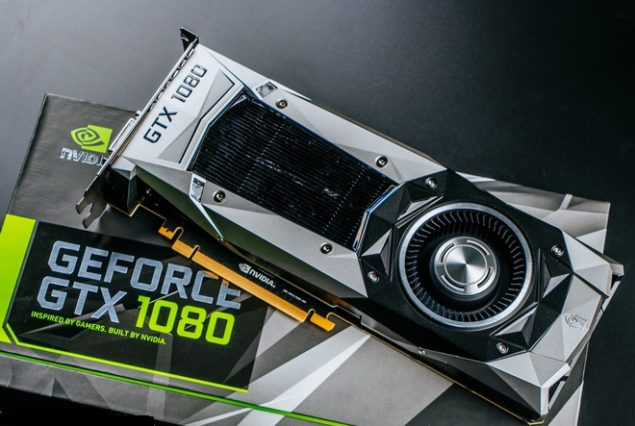
\includegraphics[width=\textwidth]{pic/gpu}\\
    		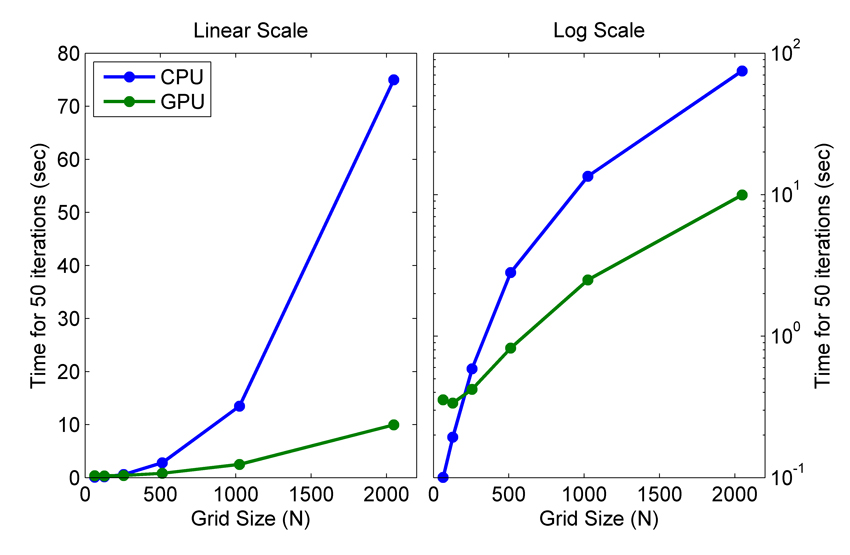
\includegraphics[width=\textwidth]{pic/gpu2}
\end{figure}
\end{minipage}
\end{frame}

\begin{frame}
\frametitle{Kitekintő: konvolúciós neuronhálók}

\begin{itemize}
  \setlength{\itemsep}{6pt}
  \item Kép: DNN probléma $\Rightarrow$ vizuális kortex
  \item CNN: speciális rétegek $\Rightarrow$ új featurek DNN-hez
  \item 3D rétegek: pixelek fölött neuronok, lokálisan kapcsolva
  \item Különböző alakokat emelünk ki a képekről
\end{itemize}

\begin{figure}[H]
	\centering
    	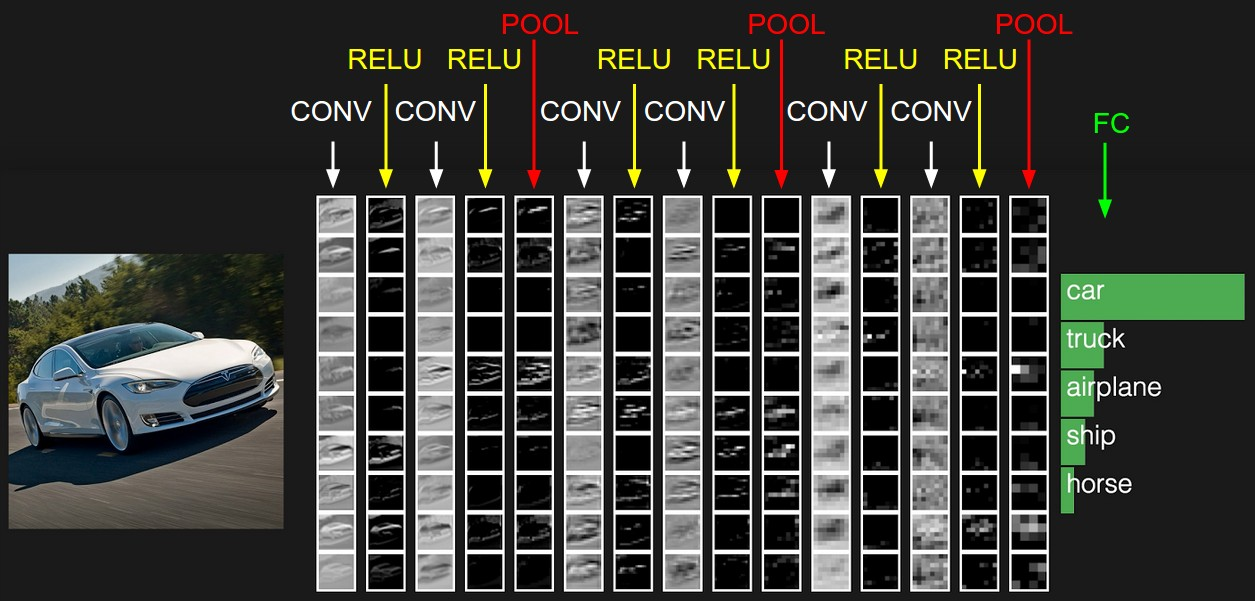
\includegraphics[width=\textwidth]{pic/cnn.jpeg}\\
\end{figure}
\end{frame}


\begin{frame}
\frametitle{Kitekintő: konvolúciós neuronhálók}
\begin{figure}[H]
	\centering
    	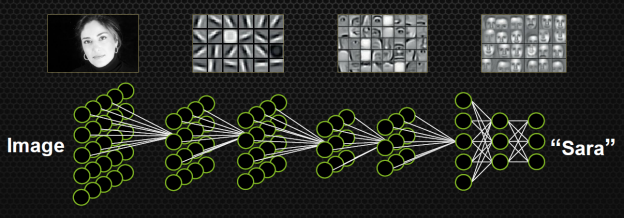
\includegraphics[width=\textwidth]{pic/cnn2}\\
\end{figure}
\end{frame}

\begin{frame}
\begin{center}
\textbf{\huge{Térjünk rá a fizikára}}
\end{center}
\end{frame}


\section{Bevezető: ROOT TMVA}
\begin{frame}
\frametitle{ROOT TMVA}
\begin{itemize}
  \setlength{\itemsep}{12pt}
  \item Toolkit for Multivariate Data Analysis (TMVA) a ROOT programcsomag része
  \item Célja: ML könyvtár biztosítása a fizikusok számára, megszokott környezetben
  \item Nem csak neuron hálókat biztosít (pl. boosted decision tree)
  \item Klasszifikáció mellett regressziót is támogat, de erről nem beszélek
  \item Alapvetően két osztály amit a TMVA névtérből kívülről használunk:
  	\begin{itemize}
  	  \setlength{\itemsep}{6pt}
  		\item TMVA::Factory: ML módszerek elérése
  		\item TMVA::DataLoader: adatok elérése
  	\end{itemize}
\end{itemize}
\end{frame}


\section{Higgs adatszett}
\begin{frame}
\frametitle{Higgs bozon keresés}
\begin{itemize}
  \setlength{\itemsep}{12pt}
  \item Feladat: Higgs bozon keresése eseményekben
  \item Nem látjuk csak a bomlás termékeket
  \item Lehetséges bomlás: $H^0\rightarrow \gamma\gamma/Z^0Z^0\rightarrow e^+e^-\;+\;e^+e^-$ (elektron párok cserélhetők müonra), ...
  \item Csak a végkimenetelt látjuk, más folyamat is produkálhat hasonló kimenetet
  \item Meghatározzunk sok fizikai paramétert (energiát, szögeket, pszeudorapiditást): ezek alapján mondjuk meg, hogy Higgs bomlás történt-e
  \item DNN-t taníthatunk be a felismerése
\end{itemize}
\end{frame}

\begin{frame}
\frametitle{Higgs adatszett}
\begin{itemize}
  \setlength{\itemsep}{18pt}
  \item CERN Opendata program keretében tanuló adatszet
  \item 5829123 esemény, 800MB
  \item 21 feature
  \item Signal: Higgs bomlás
  \item Background: nem Higgs bomlás
\end{itemize}
\end{frame}

\begin{frame}
\frametitle{Higgs adatszett}
\begin{figure}[H]
	\centering
    	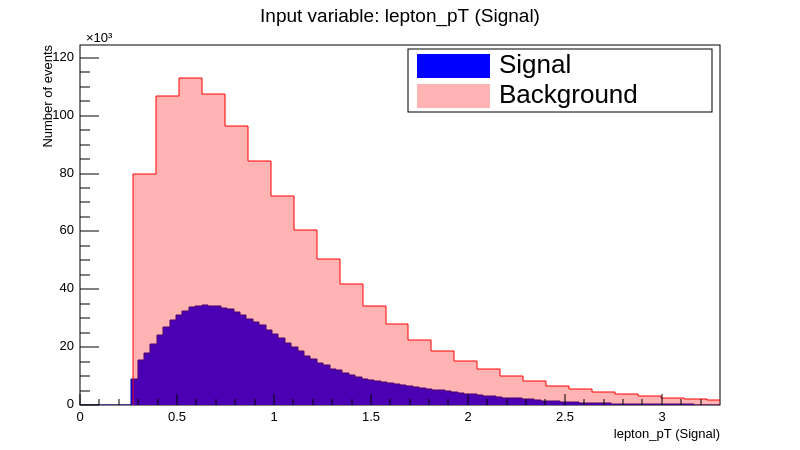
\includegraphics[width=\textwidth]{pic/higgs/1}
\end{figure}
\end{frame}
\begin{frame}
\frametitle{Higgs adatszett}
\begin{figure}[H]
	\centering
    	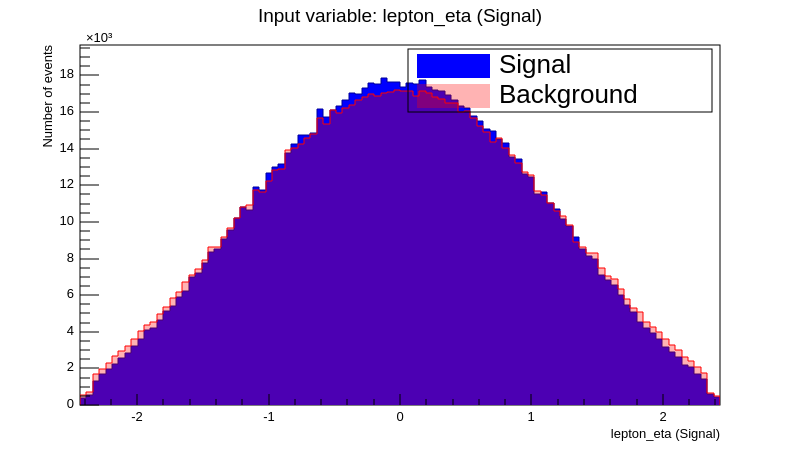
\includegraphics[width=\textwidth]{pic/higgs/3}
\end{figure}
\end{frame}
\begin{frame}
\frametitle{Higgs adatszett}
\begin{figure}[H]
	\centering
    	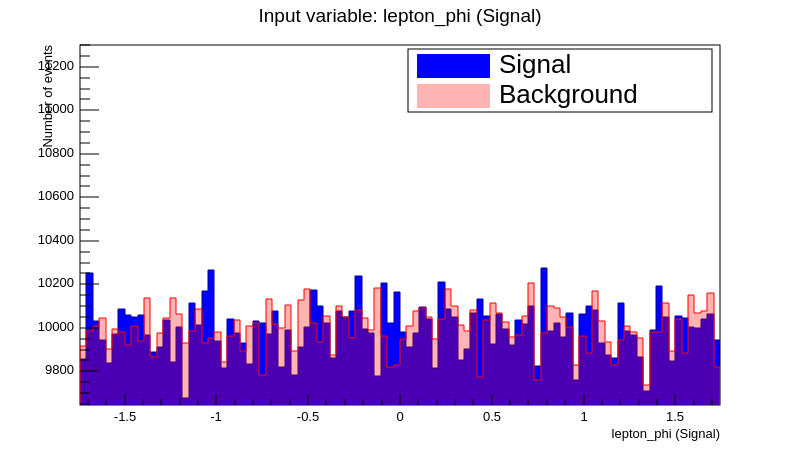
\includegraphics[width=\textwidth]{pic/higgs/4}
\end{figure}
\end{frame}
\begin{frame}
\frametitle{Higgs adatszett}
\begin{figure}[H]
	\centering
    	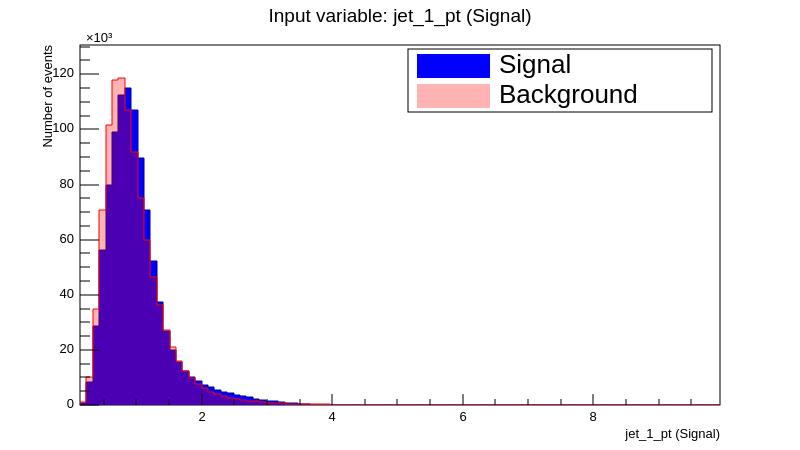
\includegraphics[width=\textwidth]{pic/higgs/5}
\end{figure}
\end{frame}

\begin{frame}
\frametitle{Higgs challenge: \url{https://www.kaggle.com/c/higgs-boson}}
\begin{itemize}
  \setlength{\itemsep}{18pt}
   \item Ki tanítja be a legjobb modellt?
  \item $\tau\tau$ bomlások megtalálása
  \item Modellt beküldve: új eseményeken teszt $\Rightarrow$ jól általánosít-e a modell?
  \item Nyertes: 
  	\begin{itemize}
  	  \setlength{\itemsep}{6pt}
  		\item 70 db. 3 rejtett rétegű, rétegenként 600 neuronos hálózat
  		\item 2-fold cross-validation
  		\item 35 random keverés az adatokon
  		\item GTX Titan GPU (mérések CPU párhuzamosan 10x lassabb)
  		\item Tanulás: 1 nap (1 háló, szimpla pontossággal csak 15 perc)
  	\end{itemize}
\end{itemize}
\end{frame}
\section{Analízis folyamata}
\begin{frame}
\frametitle{Analízis folyamata}
\begin{itemize}
  \setlength{\itemsep}{24pt}
\item \url{https://github.com/qati/Presentations/blob/master/seminar.ipynb}\newline
\item \url{http://nbviewer.jupyter.org/github/qati/Presentations/blob/master/seminar.ipynb}
\end{itemize}
\end{frame}


\end{document}

